\documentclass[11pt,a4paper,twoside]{article}

\newcommand{\student}{I. Leben}
\newcommand{\topic}{Random Access Rendering of Animated Vector Graphics Using GPU}

\usepackage{times}
\usepackage{a4wide}
\usepackage{fancyheadings}

\renewcommand{\leftmark}{\student}
\renewcommand{\rightmark}{\topic}

\usepackage{amsmath}
\usepackage{graphicx}
\usepackage{subfigure}
\usepackage{verbatim}
\usepackage{moreverb}

\newenvironment {code}{\footnotesize}{\normalsize}

\begin{document}

\title{{\sc \topic}}
\author
{
{\sc \student}
\\[3mm] {\bf Supervisor:} {\sc G. Leach}
\\[5mm] Honours Thesis
\\[5mm] School of Computer Science and Information Technology
\\ RMIT University 
\\ Melbourne, AUSTRALIA
}
\date {October, 2010}
\maketitle

\begin{abstract}
Efficient random access to image data allows texture mapping of images onto curved surfaces to be accelerated by the GPU. This property has traditionally been associated with raster images, whereas a typical vector image representation cannot be efficiently interpreted at an arbitrary point by the established graphics pipeline. Recent research has allowed texture mapping of vector images by taking advantage of the programmable stages of the GPU. However, the new rendering approach introduces an expensive preprocessing step running on the CPU. In this thesis we investigate techniques to fully accelerate vector image rendering and texture mapping on the GPU, including the preprocessing steps. We present an alternative localised vector image representation and an efficient parallel encoding algorithm, achieving great performance improvements compared to a sequential CPU implementation and allowing random access rendering of animated vector images, where continuous preprocessing is required.
\end{abstract}

\newpage
\tableofcontents
\newpage

\pagestyle{fancy}

\section{Introduction}

Random access rendering is a method whereby the colour of an image is computed at an arbitrary image space coordinate in an arbitrary order. Efficient random access to image data is a requirement for texture mapping and has traditionally been associated with raster images. The definition of a raster image as a grid of coloured pixels lends itself perfectly to the random access scheme. However, the main drawback is the artifacts such as jagged or blurred edges arising from missing detail in information when the image is scaled.

In contrast, vector graphics use mathematical equations and shapes to describe coloured regions. Such a definition allows scaling of a vector image while retaining sharp edges at colour discontinuities. As illustrated in Figure~\ref{fig:random_access_vector}, in order to classify a point as inside or outside a vector shape, we need to consider all of its primitives. Moreover, when rendering a small portion of a shape under large zoom, the parts outside of the visible area still need to be processed, adding to unnecessary overhead as the zoom factor increases. This makes straightforward approaches to random access inefficient and has until recently prevented the use of vector images as textures.


\begin {figure}
	\centering
	\includegraphics[width=1.0\columnwidth] {figures/tiger_zoom} \label{fig:tiger_zoom}
	\caption {Vector image (top row) retains sharp colour discontinuities even at large zoom, while raster image (bottom row) suffers from noticeable artifacts.}
	\label {fig:zoom}
\end {figure}

Applications of vector graphics are many, ranging from high detail maps to general scalable user interfaces.  An efficient random access algorithm would further broaden the usability of vector images. Regions of a map outside of the view could be efficiently discarded as the user zooms in on a particular detail. Graphical user interfaces could be mapped onto surfaces in 3D space allowing new ways of navigation and better screen estate management.

Historically, Graphics Processing Units (GPUs) have specialised into rendering of triangle primitives and have no built-in support for rasterization of curved shapes present in vector images. Nonetheless, dependency on the triangle-based rasterization has been alleviated by the increase in GPU programmability. Recently, \cite{NehabHoppe08} have developed a rendering technique that evaluates vector shapes directly in the programmable stages of the GPU, after localising the vector data in an expensive preprocessing step on the CPU. This allows efficient random access, but limits the use to static non-animated graphics.

An important thing to consider is the paradigm shift taken by an approach such as \cite{NehabHoppe08}. The traditional graphics pipeline starts with triangle and line primitives and rasterizes them into the framebuffer. Where primitives overlap, this results in multiple executions of the same processing instructions for a single pixel with regard to a different primitive. In contrast, the approach being discussed preprocesses the entire set of primitives in the scene to build a look-up data structure. In the final rendering stage, all the primitives affecting a given pixel can be looked up efficiently in a single execution of processing instructions to determine the colour of the pixel. It is important to note that such an approach increases the per-pixel processing complexity, but is facilitated by the recent advance in graphics hardware architecture.

\begin {figure}
	\centering
	\includegraphics[width=0.60\columnwidth] {figures/random_access_vector}
	\caption {Straightforward approaches to random-access rendering of vector images are inefficient. To find the colour of one textured pixel on the screen, all the segments of the shape need to be processed.}
	\label {fig:random_access_vector}
\end {figure}

The focus of this research is to extend the above approach by investigating alternative vector image data structures and preprocessing techniques, suitable to parallelisation and acceleration via the GPU. Our goal is to implement the entire rendering process, including the preprocessing steps, on the GPU. By taking advantage of the parallel architecture, great improvement in performance is achieved, allowing application to animated vector images where continuous preprocessing is required.

In general, this thesis investigates the following questions:

\begin {enumerate}
\item
How to efficiently accelerate vector image localisation using the parallel architecture of the GPU?
\item
Is there an alternative localised vector image representation, more suitable to parallel encoding and rendering?
\item
What are the performance gains of a parallel preprocessing algorithm compared to a sequential CPU implementation?
\item
What degree of vector data localisation provides an optimal balance between preprocessing and rendering time?
\item
What is the benefit of vector data localisation with regard to animated vector graphics where continuous preprocessing is required?
\end {enumerate}

\section {Background}
\subsection {Vector Image Definition}

A vector image is a set of vector shapes, each defined as an open or closed spline of straight line and curved segments. Closed shapes can be filled, meaning the spline defines a border between the exterior and the coloured interior of the shape. Shapes can also be stroked, meaning the boundary has a visible thickness. For practical purposes, stroked shapes can be adequately approximated by another more complex vector shape describing the resulting outline of the thick line, thus reducing the definition to closed, filled shapes.

The interior of the filled shapes is determined according to the value called \emph{winding number}. For any point, the winding number represents the total number of times that the curve travels around the point. Clockwise movement counts as positive whereas anticlockwise movement counts as negative. Figure~\ref{fig:winding} shows examples of points in curves and their respective winding numbers. Note that one shape can consist of multiple contours in which case the winding number is the sum of the individual winding numbers of all the contours.

There are two common rules for determining the interior of a shape, namely \emph{even-odd} and \emph{non-zero}. The former classifies the areas with an odd winding number as interior while the latter considers any area with a winding number different than $0$ to be inside. Depending on the number of contours and their orientation, a shape might have a different or equal appearance with different fill rules.

\begin {figure}
	\centering
	\subfigure [] { \includegraphics [width=0.13\columnwidth] {figures/winding1} \label{fig:wind_a}}
	\hspace{0.5cm}
	\subfigure [] { \includegraphics [width=0.13\columnwidth] {figures/winding2} \label{fig:wind_b}} \\
	\hspace{0.5cm}
	\subfigure [] { 
\includegraphics [width=0.13\columnwidth] {figures/fill_rule_even_odd_1} \label{fig:wind_c}}
	\hspace{0.5cm}
	\subfigure [] { 
\includegraphics [width=0.13\columnwidth] {figures/fill_rule_non_zero_1} \label{fig:wind_d}}
	\hspace{0.5cm}
	\subfigure [] { 
\includegraphics [width=0.13\columnwidth] {figures/fill_rule_any_2} \label{fig:wind_e}}
	\caption
		{\subref{fig:wind_a} a shape consisting of a single contour
		\subref{fig:wind_b} a shape consisting of two contours with opposite orientation
		\subref{fig:wind_c} shape A using even-odd fill rule;
		\subref{fig:wind_d} shape A using non-zero fill rule;
		\subref{fig:wind_e} shape B appears the same using both fill rules.}
	\label {fig:winding}
\end {figure}

\subsection{Evaluation of Spline Segments}

Individual segments of a vector spline are most commonly defined using B\'{e}zier curves of first to third degree, as described in \cite{Farin02}. In general a B\'{e}zier curve of degree $n$ is defined as follows:
\[ \mathbf{B}(t) = \sum_{i=0}^{n} \mathbf{b}_{i,n}(t)\mathbf{P}_i, \quad t \in [0, 1] \]
where the points $\mathbf{P}_i$ are called \emph{control points} of the B\'{e}zier curve and the polynomials
\[ \mathbf{b}_{i,n}(t) = \binom{n}{i} t^i (1 - t)^{n-i}, \quad i = 0, ... n \]
are known as Bernstein basis polynomials of degree $n$ with the following property:
\[ \sum_{i=0}^{n} \mathbf{b}_{i,n}(t) = 1, \quad t \in [0, 1] \]
meaning that the sum of all the polynomials of the same degree is always $1$. The B\'{e}zier curve equation therefore interpolates between the given control points according to the parameter $t$, beginning exactly at $\mathbf{P}_0$ and ending exactly at $\mathbf{P}_n$. A curve of degree $n$ has $n+1$ control points. A  B\'{e}zier curve of degree $1$ is essentially a straight line. Consecutive spline segments share a control point where one ends and the next one begins. The ordered set of control points of all the segments defines the \emph{control polygon} of the spline as shown in figure~\ref{fig:spline}.

A simple way of finding a point on the  B\'{e}zier curve at an arbitrary parameter value is to substitute the value into every basis function, compute the products with the respective control points and add them together. While straightforward, this approach is not numerically stable. Instead, as described in \cite{Boehm99} we can evaluate the points on the curve by recursive subdivision of the sides of its control polygon. This technique, known as \emph{de Casteljau's algorithm} reduces numerical errors during the course of evaluation.

\subsection{Winding Number Evaluation}
\label{sec:winding}

The B\'{e}zier curve equations can also be used to evaluate the winding number of any point with regards to a vector spline. We start by casting a ray from the point in an arbitrary direction. Based on the \emph{Jordan Curve Theorem}, the point is found to be inside the polygon, if the ray crosses an edge of the polygon an odd number of times. Counting the number of intersections gives a value known as the \emph{crossing number}. Now, by checking the direction of the intersecting edge, we instead add $+1$ for every left-to-right crossing and $-1$ for every right-to-left crossing. The resulting value is the winding number of the point.

Imagine the ray is being cast from point $P(x,y)$ horizontally in the positive direction of the $x$ axis. We can find an intersection with any segment of the spline by finding the roots $t_i$ of the equation $y = y(t)$ where $y(t)$ is the linear or higher order polynomial describing the spline segment. When $t \in [0,1]$ and $x < x(t)$, the ray intersects the segment.

\begin {figure}
\centering
\begin {minipage}[b]{0.45\linewidth}
	\centering
	\includegraphics [width=0.8\columnwidth]{figures/spline}
	\caption {A closed spline (red) consisting of two line segments and two cubic B\'{e}zier curve segments with its control polygon (black).}
	\label {fig:spline}
\end {minipage}
\hspace{0.5cm}
\begin {minipage}[b]{0.45\linewidth}
	\centering
	\includegraphics [width=0.8\columnwidth]{figures/ray}
	\caption {The direction of the intersections between a horizontal ray and the segments of a spline count towards the winding number of the point.}
	\label {fig:ray}
\end {minipage}
\end {figure}

Obviously, the winding number at any point depends on the geometry of the entire shape outline. More precisely, to evaluate the winding number of a single point, all the segments of the shape to the right of this point need to be identified and checked for horizontal ray intersection. It is this requirement that poses the greatest obstacle when designing an efficient random access rendering algorithm.

\begin {figure}
	\centering
	\includegraphics [width=1.0\columnwidth]{figures/gfx_pipeline}
	\caption {In traditional graphics pipeline, transformed vertices are assembled into one of the three primitive types and then rasterized into the framebuffer.}
	\label {fig:gfx_pipeline}
\end {figure}

\subsection{Traditional Graphics Pipeline}

Modern display devices require input in the form of a grid of colour values, called a \emph{raster}. A colour value in a raster is called a \emph{pixel}. For a graphical object to be displayed, the pixels covered by its shape need to be determined in a process called \emph{rasterisation} and the colour values in the display raster changed accordingly. The architecture of modern GPUs is optimised for rasterisation of three types of primitives: points, lines and triangles. The roots of this design reach into the early history of computer graphics when parallel computing architecture was not as powerful and programmable as today. Triangle rasterisation coupled with texture mapping of raster images was much simpler to implement in hardware compared to direct evaluation of higher order mathematical equations. Thus more complex shapes have to be converted into the basic primitives by tesselation, in order to accommodate and benefit from hardware-accelerated rendering.

Figure~\ref{fig:gfx_pipeline} shows how a traditional graphics pipeline processes the data. The input comes in the form of vertices which can carry multiple attributes, such as vertex coordinate, texture coordinate and colour. The pipeline itself also has a set of attributes which represent its state. The state governs the processing of the input data and can be modified by the drawing commands. It includes important processing information, such as the vertex transformation matrix and the type of primitive for the current set of vertices.

The pipeline consists of three stages. The vertex transformation stage applies the transformation matrix defined in the pipeline state to the vertex coordinates. The primitive assembly stage combines the transformed vertices into one of the three basic primitive types, as defined in the pipeline state. The rasterization stage determines the pixels covered by each primitive and computes the interpolated values of the vertex attributes at every pixel. Finally, the resulting colour at each pixel is written into a temporary memory block called \emph{framebuffer}. When the entire image of one frame is constructed, the colour data is copied from the framebuffer into the actual display raster.

\subsection{Texture Lookups}

There are two common ways of determining the final pixel colour. As shown in Figure~\ref{fig:gfx_pipeline}, a colour value can be attached to each vertex as one of its attributes and interpolated across the primitive. Alternatively, every vertex can have a texture coordinate attached. The interpolated texture coordinate at every pixel is used to perform a lookup into a texture image, residing in video memory of the GPU. The lookup applies the colour of the texture at the point of texture coordinate to the pixel and might include some form of filtering to smooth out the colour values of adjacent pixels. This process is illustrated in Figure~\ref{fig:texturing}. A group of textured triangles small enough to approximate a curved surface can give an impression of the texture image being mapped onto an arbitrary surface.

Due to parallel architecture of the rasterization stage, every pixel is processed separately and the order of coordinates in the texture lookups is arbitrary. In order to be usable as a texture an image must offer efficient random access to its data. To this end, raster images have long been used for texturing. If the colour tuples are laid out in row-major order, the following simple equation suffices to compute the memory location of a pixel within the raster data:
\[ L = Y * W + X \]
where \emph{(X,Y)} is the texture coordinate and \emph{W} is the width of raster image in pixels. Once the memory location is computed, the texture colour can be read directly from the raster grid and applied to the pixel being textured.

On the other hand, vector images do not offer such a simple and efficient colour lookup. As discussed in previous sections, the colour at an arbitrary coodinate in image space depends on the winding number of that point with regards to every shape in the image. Furthermore, every winding number in turn depends on every segment of the respective shape. In order to use vector images as textures some preprocessing needs to be done, to construct a more efficient lookup structure.

\begin {figure}
	\centering
	\includegraphics [width=0.7\columnwidth]{figures/texturing}
	\caption {The process of texturing maps the texture image onto a curved surface by interpolating the texture coordinate at every vertex across the primitive and performing a lookup at every pixel.}
	\label {fig:texturing}
\end {figure}

\subsection{GPU Programmability}
The GPU has evolved enormously in terms of speed and programmability, however the fundamental approach has not changed much, with the triangle rasterisation unit remaining a core built-in component. Nonetheless, the increase in programmability has enabled new ways of using the GPU.

Firstly, programmers can now write code that defines the behaviour of certain stages of the rendering pipeline as exposed by the graphics APIs such as OpenGL and DirectX. The pipeline is still based around points, lines and triangles being the basic rasterizable primitives, however, custom programs for processing of vertices and pixels can be uploaded onto the hardware. Figure~\ref{fig:gl_pipeline} shows the graphics pipeline as presented by the OpenGL API. The programmable stage processing the vertices is called a \emph{vertex shader}, while the pixel processing stage is named a \emph{fragment shader}.

The programmable stages can be used to enhance the traditional pipeline by implementing arbitrary transformation of the vertex input or alternative means of computing the output pixel colour. More importantly, they allow the use of GPU processor as a generic processing unit, an approach known as \emph{General Purpose GPU processing} (GPGPU). Arbitrary input data can be encoded into vertices and then decoded and processed by the shading program. The ability to perform texture lookups at any point in a shading program allows arbitrary data encoded into textures to be read directly from the GPU memory. The option to render into the raster of a texture image, rather than the display raster, allows generic output to be encoded and written out as colour values.

Moreover, new programming interfaces such as CUDA and OpenCL have emerged that expose the GPU hardware as a generic multi-core computing device. This approach is known as \emph{GPU Computing}. These APIs  are completely devoid of any graphics-related paradigms, so there is no need to encode the data into graphical entities such as vertices and textures. Nonetheless, the results of the computation are often used for graphical purposes or end up being visualised via traditional rendering pipeline.

\begin {figure}
	\centering
	\includegraphics [width=1.0\columnwidth]{figures/gl_pipeline}
	\caption {OpenGL rendering pipeline. Programmable parts are coloured in blue.}
	\label {fig:gl_pipeline}
\end {figure}

\subsection{Recent Advances in the GPU Architecture}

With the increasing use of the GPU for general-purpose computation and the shift of the CPU towards multi-core computing, the architectures of the two processing units are starting to converge. On the one hand, the number of cores on the CPU increases with every generation. On the other hand, recent GPU architectures include features that were previously only found on a CPU.

NVIDIA has recently released a new generation of GPUs code named \emph{Fermi}. Among other improvements, the new architecture introduced two very important features for our research: global memory space and a unified cache architecture. A new set of 64-bit addressing instructions allows C-style memory pointers to be used in shader code. The cache architecture ensures coherence in memory accesses between multiple shading threads, allowing data structures in the global memory to be shared between parallel executions of shader code. Concurrent access can be synchronised via atomic operations, which received a significant performance improvement compared to previous GPU generations.

Although these changes are mostly targeted towards GPU Computing, some of them are exposed to the graphics pipeline as well. The OpenGL API allows new features to be brought in through third party \emph{extensions}, which accelerate the evolution of the interface even before the new features are approved as part of the core API. With the new architecture, NVIDIA also released extensions to OpenGL which take advantage of the new GPU capabilities in order to increase the versatility of the graphics pipeline.

Extensions {\tt EXT\_shader\_image\_load\_store} and {\tt NV\_shader\_buffer\_store} add new features to the shading language, allowing writes to arbitrary locations in the GPU memory. The former achieves this by allowing a texture image to be bound as a new type of rendering target, thus limiting the valid write locations to a subset of memory. The latter enhances the shading language with C-style pointers, through which the memory can be read or written at any location within the global memory space. Both extensions add new built-in functions to the language to perform atomic read and write operations.

The reason these two extensions are so important is they allow more complex data structures to be constructed in the GPU memory. Previously, the output of a fragment shader had a fixed location in the target framebuffer at the coordinate of the respective pixel. With the new memory access functions, a shading program can lay out the data structures in memory much like a typical CPU program would. By using these extensions, our preprocessing implementation can build an efficient vector image lookup structure in parallel from multiple executions of the shading program.

\section {Previous Work}

\begin {figure} [ht]
	\centering
	\subfigure[Subdivision]{\label{fig:DeCasteljau}\includegraphics [width=0.3\columnwidth] {figures/DeCasteljau}}
	\hspace{2.0cm}
	\subfigure[Tesselation]{\label{fig:tesselation}\includegraphics [width=0.3\columnwidth] {figures/tesselation}}
	\caption {Traditional CPU renderer subdivides curves into straight line segments and then tesselates the shape interior into triangles.}
	\label {fig:cpu}
\end {figure}

In a typical CPU implementation of a vector graphics renderer, every spline is first approximated by linear segments. Intermediate points on the curved segments can be obtained in a straightforward manner by curve evaluation at a fixed step. Alternatively, the process can be optimised via adaptive algorithms which generate less points in the straight regions and more points in the regions of higher curvature. Common approaches include forward difference evaluation and recursive subdivision based on de Casteljau algorithm. The interior of the resulting piecewise linear polygon is triangulated according to the fill-rule applied to the shape. Finally, the triangles are rasterized into the framebuffer. Figure~\ref{fig:cpu} illustrates the process of subdivision and tesselation.

Unfortunately, the known curve subdivision and polygon triangulation algorithms are expensive in terms of required processing time compared to the final rendering of the image. Moreover, they are inherently sequential, which means they cannot be efficiently parallelised and therefore cannot take advantage of the GPU.

\subsection {Forward Rendering Approaches}

\cite{LoopBlinn05} have developed an approach where the implicit equation of quadratic curves is evaluated directly in the fragment shader to perform inside/outside classification. They start by observing that ``the implicit form of any rational parametric quadratic curve is a conic section; and that any conic section is the projected image of a single canonical parabola." They show that a quadratic curve with control points $(0,0)$, $(0.5,0)$, and $(1,1)$ plots the quadratic curve $v = u^2$ exactly. They assign these points as the $(u,v)$ texture coordinates to the vertices of a triangle. Suppose the vertices are the control points of another arbitrary quadratic curve. As the hardware interpolates the texture coordinates across the triangle, it essentially projects the quadratic curve from texture space into screen space. They determine if the pixel is inside or outside the curve by evaluating $f(u,v) = u^2 - v$ in a pixel shader program. If $f(u,v) < 0$ then the pixel is inside the curve, otherwise it is outside.

\begin {figure}
	\centering
	\includegraphics [width=0.5\columnwidth] {figures/loop_blinn}
	\caption {A quadratic curve is projected from texture space into screen space via coordinate interpolation. (Image source: \cite{LoopBlinn05}) }
	\label {fig:loop_blinn}
\end {figure}

\begin {figure}
	\centering
	\includegraphics [width=0.5\columnwidth] {figures/kokojima}
	\caption {Stencil-buffer rendering technique based on Jordan Curve theorem avoids the need for triangulation of shape interior. (Image source: \cite{Kokojima06}) }
	\label {fig:kokojima}
\end {figure}

This removes the need for curve subdivision, but the interior of the shape still needs to be triangulated. \cite{Kokojima06} combine the projective rendering of the quadratic curves with a stencil polygon rendering technique. First, an arbitrary pivot point is selected. For each linear segment a triangle is drawn with one of its vertices at the pivot point and the other two at the vertices of the line segment. For each quadratic segment a triangle is drawn between the pivot point and the first and the last control point, skipping the middle control point. Additionally, a triangle is drawn for each quadratic curve, discarding the pixels based on the projective technique of \cite{LoopBlinn05}. For every pixel drawn, the binary value in the stencil buffer is inverted. After all the triangles have been drawn, the values in the stencil buffer essentially represent the crossing number for every point as if the intersection ray was cast towards the pivot point. This allows the pixels in the framebuffer to be coloured according to even-odd fill rule.

\subsection {Random Access Rendering by Image Localisation}

\begin {figure}
	\centering
	\includegraphics [width=1.0\columnwidth] {figures/nehab_hoppe}
	\caption {Random access rendering introduces a new paradigm in vector image rendering. (Image source: \cite{NehabHoppe08}) }
	\label {fig:nehab_hoppe}
\end {figure}

The algorithms described so far enable efficient rendering of animated vector graphics. However, they are strongly based on the traditional primitive rasterization pipeline. As such, the rendered image can only be transformed by transforming the vertices of the triangle primitives before they are rasterized. Instead, we are aiming to use vector images as textures and map them onto other surfaces. As discussed previously, texture lookups follow a random access scheme, where the pixel colours are queried at an arbitrary coordinate within the image space in an arbitrary order. To achieve this, we need to construct an efficient lookup structure, that will allow us to evaluate the winding number of any point with respect to any vector shape from within the fragment shader.

\cite{NehabHoppe08} presented an approach to this problem that localises the vector image representation to coarse lattice cells in a preprocessing step implemented as a sequential CPU algorithm. Each cell contains a localised description of the graphics primitives it overlaps. This information is encoded into a GPU texture and interpreted by the fragment shader. For every fragment, the vector data is read from the lattice cell that the texture coordinate falls in. The winding number is calculated using the ray-casting intersection technique, but thanks to the localisation, only the segments overlapping the cell need to be considered. They observe that increasing the lattice resolution decreases the number of spline segments to intersect per pixel, as long as the detail in the image is fairly uniform. This in turn reduces the rendering time and increases the achievable rendering framerate. However, they find that the preprocessing takes too long for real-time use which prevents their approach to be used with animated images.

The above approach represents an important paradigm shift in vector image processing. Previous rendering techniques used vector image data as direct input to the traditional pipeline. Control vertices of vector curves were represented as vertices of basic graphics primitives and the primitive rasterization stage was cleverly enhanced with the specialized shading programs to perform the inside / outside classification of every pixel. In contrast, the image localisation approach does not represent any part of the vector image data using traditional graphics pipeline entities. A GPU texture is used merely as a memory buffer to contain encoded vector data and the fragment shader is used as a generic unit of computation that performs a look up into the encoded data and emits the resulting pixel color.

\section {Our Approach}

In order to extend the random access rendering technique by \cite{NehabHoppe08} to animated vector images, the preprocessing step that constructs the lookup data structure needs to be accelerated. Their localised image representation is organized into grid cells, so it lends itself directly to a parallel encoding algorithm, meaning it can benefit from the parallel architecture of the GPU.

However, their "fast lattice-clipping algorithm" involves certain steps which cannot be efficiently parallelised. To preserve the winding number within a cell, their algorithm creates auxiliary segments on the right boundary of each cell. The direction of the auxiliary segments affects the resulting winding number and depends on the segments in other cells, to the right of the cell in question. Therefore, for every segment crossing a cell, the winding number needs to be integrated into the cells to its left. The dependency of each cell on the contents of other cells makes it challenging to devise a parallel localisation algorithm.

To avoid bottlenecks in our approach, we develop an alternative pivot-point (PP) localised image representation in an effort to minimise inter-cell dependencies and allow our encoding algorithm to take maximum advantage of the parallel GPU architecture. We also present an adjusted rendering algorithm that utilizes PP image representation for texture mapping.

\subsection {Pivot-Point Localised Image Representation}

\begin {figure}
\centering
\begin {minipage} [b] {0.45\linewidth}
	\centering
	\includegraphics [width=0.6\columnwidth]{figures/ray_our}
	\caption {Starting from a known winding number, the winding number of adjacent regions can be determined by a single crossing of an edge.}
	\label {fig:ray_our}
\end {minipage}
\hspace{0.5cm}
\begin{minipage} [b] {0.45\linewidth}
	\centering
	\includegraphics [width=0.6\columnwidth]{figures/cell}
	\caption {Casting a ray from the pivot point and intersecting the segments in the cell gives the winding number of any other point within the same cell.}
	\label {fig:cell}	
\end {minipage}
\end {figure}

There are two main requirements for our localised representation: (i) it must exhibit a high degree of localisation to allow efficient random-access and (ii) it must be obtainable via some process which can achieve a high degree of parallelism. Like \cite{NehabHoppe08}, we create a coarse grid across the original vector image. However, our approach differs in the contents of the grid cells. 

We start by observing that the winding number of any region in a vector shape can be determined by a single crossing of an edge, as long as the winding number of another adjacent region is known. As shown in Figure~\ref{fig:ray_our} it is possible to move from one region to another, adjusting the winding number according to the direction of the crossing edge and thus finding the winding number of every region.

We take advantage of this observation by assigning a pivot point to every cell, with its location implicitly defined as the center of the cell. We find the winding number of the pivot point in the preprocessing step and then use it as the source for ray-casting, similar to how the forward rendering technique of \cite{Kokojima06} uses one of the control points as the pivot point for construction of auxiliary triangles.

We adjust our rendering algorithm accordingly. While \cite{NehabHoppe08} cast a horizontal ray in the positive $x$ direction, we cast a ray from the pivot point $P$ of the cell in an arbitrary direction towards any other point $W$ in the cell for which the winding number is needed. The intersections of the ray with vector segments of the shape give the change in winding number of $W$ from the original winding number of $P$. Note that only the segments within the same cell as $P$ and $W$ need to be checked for intersection, as those are the only segments that can potentially stand in between the two points. Therefore, the number of segments that need to be intersected effectively decreases with the increase in grid resolution, thus satisfying requirement (i) for our localised representation.

In contrast to cell contents of an AS representation, the pivot winding number in PP representation only depends on the geometry of the shape and not the resulting contents of other cells in the grid. This makes our representation more suitable to a parallel construction algorithm. As explained in Section~\ref{sec:winding}, finding the winding number at an arbitrary location on a point-by-point basis is not efficient. However, the subsequent sections show that it is possible to find the winding numbers for a set of points efficiently with a parallel algorithm, as long as the coordinates of the points are known in advance. Since locations of cell pivot points become known as soon as the grid resolution is chosen, our localised representation satisfies requirement (ii) set above.

Our PP representation of a vector image thus consists of a set of grid cells containing a pivot winding number and the list of intersecting spline segments. In contrast to AS representation, no additional auxiliary segments are required, resulting in a smaller number of segments per grid cell.

\subsection {Image Pipeline}

We split our image processing pipeline into two stages: encoding and rendering. The purpose of the encoding stage is to convert the original vector image data into a localised representation. This stage performs all the preprocessing required so that the resulting lookup structure can be directly used for rendering. As long as the image data does not change, only the rendering stage needs to be invoked in order to display the image. When the image is animated, the encoding stage is invoked on every frame to rebuild the lookup structure before the rendering stage.

The following sections describe our encoding and rendering algorithms in detail. In order to be able to compare the performance of the two different localised representations, we implemented the encoding pass and the rendering pass for both our PP representation as well as the AS representation by \cite{NehabHoppe08}. The algorithms are mostly similar for both image representations, except where we explicitly mention the differences.

Despite the output of the encoding stage being used for rendering purposes, the encoding algorithm cannot be modeled directly by the traditional graphics pipeline. Like \cite{NehabHoppe08}, we use a GPGPU approach rather than a fully generic GPU Computing approach, meaning the steps of the algorithm are expressed in terms of graphical constructs. The main reason for this choice is that the GPU Computing is still rapidly evolving, with tools maturing, and that to our knowledge the GPGPU approaches still performed better.

%The input to the algorithm is the original vector image description consisting of a set of control points, segment types and colour for every shape. The output is a specialised version of that description, localised to every grid cell and encoded into its respective data stream.


%\subsection{Memory interface}
%
%The input to the encoding algorithm is given in the vertex buffers uploaded onto the GPU. The output is also stored in the GPU memory and directly reused by the rendering stage. Since the entire process of encoding and drawing is repeated in every frame, the output buffers can be reused between multiple images. This means the upper bound on the memory used by our approach is equal to the memory requirements of the largest image ever being drawn and does not increase when additional vector images are used in the same scene.
%
%Our GPU implementation of the image encoding would not be possible without read and write access to an arbitrary location in the GPU memory. To achieve that, we used the previously described {\tt NV\_shader\_buffer\_store} OpenGL extension, only available on most recent hardware. An additional advantage of this extension is the ability to cast memory pointer types and thus view parts of the same block of memory as a different data type. This allows the memory to be viewed through C-like structures defined in the shader code and thus store integer and floating point numbers of different bit sizes next to each other. Unfortunately, our time constraints did not allow us to investigate the potential advantages of such an approach. Instead, we allocate all the GPU buffers as a 32-bit integer or floating point array and always use them through the pointer of the same respective type. It might also be worth investigating the performance and memory advantages of using 16-bit precision variables in various parts of our data structures. This was left for future work.

\subsection{Intermediate and Output Memory Buffers}

\begin {figure}
	\centering
	\includegraphics[width=0.4\columnwidth] {figures/data_buffers}
	\caption {Three buffers used by the encoding algorithm. The main indirection grid and the stream buffer are the input to the rendering pass.}
	\label {fig:data_buffers}
\end {figure}

During the execution of our preprocessing algorithm, two intermediate memory buffers are used and one output buffer shown on Figure~\ref{fig:data_buffers}. The intermediate synchronisation buffer and the grid buffer are allocated as 32-bit integer arrays. They hold counter variables which are accessed during the algorithm via atomic operations to synchronize encoding of the interleaved cell streams. The synchronisation buffer holds just a single global stream length counter. The grid buffer holds several counters for every cell of the main grid as well the smaller object grids. The purpose of each of the grid counters is described later in the algorithm details. The object grids hold their own set of these same counters which are required to be able to process segments of multiple objects simultaneously and thus maximise the achievable level of parallelism. The size of an object grid is determined by the bounding box of the respective object. However, the cells of these sub-grids are aligned with the cells of the main grid, so that the information can be assimilated and propagated to the main grid at the end of the encoding.

The stream buffer is allocated as a 32-bit floating point array. It holds the cell stream data represented as interleaved linked lists. Each cell stream belongs to one cell in the main grid and encodes the spline segments or auxiliary segments intersecting that cell. Each node of a linked list encodes the control points of a spline segment or an object info header.

\subsection {Segment Cell Stream}

The data in the stream buffer is organized into nodes of different types, inter-linked via the stream index of the first data in the node. Different nodes have different number of data values and therefore different sizes. The first value in every node defines the type of the node. The second value in every node is the link to the previous node in the same list. The following values in the node encode the control points of the line or quadratic curve segment or the properties of an object.

Such organisation allows us to interleave multiple lists within the same memory space. One list contains segments of one particular object intersecting one particular grid cell. There might be multiple objects intersecting the same cell, which results in multiple linked lists per cell. The counters in the object sub-grids are used to facilitate concurrent construction of lists for all the object within the same cell as described below.

The variables used in the list construction are the following:

\begin {enumerate}
\item
Atomic counter $L$ in the synchronisation buffer holding total stream length
\item
Atomic counter $H$ in a cell of the grid buffer holding stream index of the first node (list head)
\item
Size $S$ of the new node as number of stream words
\item
Stream index $I$ of the new node in the list
\item
Stream index $P$ of the previous node in the list
\end {enumerate}

The node insertion algorithm is as follows:
\begin{verbatimtab}[3]
	I = atomicAdd( L, S )
	P = atomicSwap( H, I )
	stream[ I ] = nodeType
	stream[ I+1 ] = P
	stream[ I+...] = additional node data...
\end{verbatimtab}

where \emph{atomicAdd} function adds the given value to an atomic counter and \emph{atomicSwap} function swaps the value of the atomic counter with the new value. Both atomic functions return the old value read prior to the modification.

\begin {figure}
	\centering
	\includegraphics[width=0.6\columnwidth] {figures/cell_stream}
	\caption {The state of the stream buffer and synchronisation counters after the first two segments of a triangle shape are processed.}
	\label {fig:cell_stream}
\end {figure}

The segment encoding pass uses atomic counter $H$ in the sub-grid of the object to which the current segment belongs. By using separate head pointers for every object, multiple linked lists per cell can be constructed concurrently, which are then assembled in another pass encoding the object info headers. The object encoding pass uses the atomic counter $H$ in the main grid, but reads the $H$ counter from respective object grid cell and stores it into the object header node. This results in a single linked list per cell of the main grid containing object headers, where each object header points to another linked list containing the object segments intersecting the cell. Figure~\ref{fig:obj_stream} illustrates one possible final structure of a stream buffer.

The final back-to-front sorting pass iterates through the object header linked list for every cell and sorts the contents of the nodes based on the index of the object in the vector image.

\begin {figure} 
	\centering
	\includegraphics[width=0.6\columnwidth] {figures/obj_stream}
	\caption {The stream buffer contains interleaved nodes of multiple linked lists. Each linked list contains segments of one particular object intersecting one particular grid cell.}
	\label {fig:obj_stream}
\end {figure}

\subsection {Encoding Input Setup}

Our encoding algorithm requires minimal setup by the CPU which includes the following steps:

\begin {enumerate}
\item
Approximate cubic curve segments with multiple quadratic segments.
\item
Compute the coarse bounding box of the entire image and every separate object based on the segment control points.
\item
Compute the memory size of the main grid and object sub-grids to format the grid memory pool.
\item
Upload the object grid offset indices and segment control points into the GPU buffers.
\end {enumerate}

The input required by every pass of our encoding algorithm is represented with the smallest number of vertices that define the respective geometry, so as to minimize the amount of data required to be sent to the GPU on every frame. Objects are represented by a line primitive extending from the minimum point to the maximum point of the object's bounding box. Straight line segments are represented directly by a line primitive. Quadratic curve segments are represented by a triangle which encodes the three control points of the curve.

Note that these input primitives are never processed by the graphics pipeline. Rather, they are only used to carry the input data to the algorithm and to trigger the pipeline execution. As described later, initial primitives are discarded by the geometry shader, after the input data is decoded.

\subsection {Encoding Algorithm}

Parallelism in our implementation is achieved by distributing the processing of geometry between multiple shader processors on the GPU with regard to segments, control points or grid cells. 

The first level of parallelism is achieved with the vertex shaders, where multiple control points are processed simultaneously. The second level of parallelism is achieved with the geometry shaders, where additional processing such as bounding box computation can be applied to multiple segments simultaneously. The third and final level of parallelism is achieved with the fragment shaders, where processing can be applied to multiple grid cells simultaneously.

A coarse description of our encoding algorithm is given in pseudocode below, excluding the details that differ between the auxiliary-segment and pivot-point representations:

\begin {code}
\begin {verbatimtab}[3]

init stream length counter to 0

for (every main grid cell)
	init main cell counters to -1
loop

for (every object)
	for (every object grid cell in bbox)
		init object cell counters -1
	loop
loop

Init object grid counters

[Sync memory]

for (every object)
	for (every line segment)
		find line bounding box
		for (every object grid cell in bbox)
			if (intersects cell)
				encode segment into cell stream
			loop
		loop
	loop
	for (every quadratic segment)
		find quad bounding box
		for (every object grid cell in bbox)
			if (intersects cell)
				encode segment into cell stream
			loop
		loop
	loop
loop

[Sync memory]

for (every object)
	for (every object grid cell in bbox)
		encode object header into cell stream
		link main grid cell to the object header
	loop
loop

[Sync memory]

for (every main grid cell)
	sort object headers in the stream back-to-front 
loop

[Sync memory]
\end {verbatimtab}
\end {code}

Note that due to the previously described parallelisms the steps of the loops actually run in parallel. Each top-level for loop is a separate rendering pass. The passes of the form
\begin{code}
\begin {verbatimtab}[3]
for (every main grid cell)
\end {verbatimtab}
\end{code}

are implemented as drawing of a rectangle over the entire main grid. The transformation matrices are set so as to match the size of a covered pixel to the size of one grid cell. This gives us $M x N$ invocations of the fragment shader, where $M x N$ is the size of the main grid. Per-cell processing is implemented in the fragment shader so that each invocation of the shader computes the results for its respective cell. The passes of the form
\begin{code}
\begin {verbatimtab}[3]
for (every line\quad segment)
	for (every object grid cell in bbox)
	loop
loop
\end {verbatimtab}
\end{code}

start off as drawing of a line or triangle primitive. The geometry shader takes in two or three control points defining the segment and computes their bounding box by combining their minimum and maximum coordinates in each dimension. The minimum coordinates are rounded down and the maximum coordinates are rounded up to the nearest grid cell. The geometry shader then discards the line or triangle primitive and emits a rectangle covering the cells within the bounding box. Again, this results in an invocation of a fragment shader for every cell that is potentially intersected by the line or quadratic segment. The passes of the form
\begin{code}
\begin {verbatimtab}[3]
for (every object)
	for (every object grid cell in bbox)
	loop
loop
\end {verbatimtab}
\end{code}

are initiated as drawing of line segments extending from the minimum to the maximum point of the object bounding box rounded to the nearest grid cell. These coordinates are precomputed in the setup stage, since they are required to format the grid memory pool. Same as in the other two cases above, the geometry shader simply discards the line segments and emits a rectangle matching the bounding box instead.

We mentioned previously the cache hierarchy introduced in the latest GPU architecture. Due to multiple levels of cache, the concurrent memory access might result in memory discrepancies as seen by the processors from different processing groups. To avoid this, an explicit function call needs to be issued to synchronise the memory across all the processors. It is important to note that none of the points of memory synchronisation are inside a loop, which means the number of required synchronisations is fixed and does not increase with the complexity of the input data. 

This was especially challenging to achieve on the level of objects when an image consists of more than one shape of different colors. The linked lists of segments for each object need to be separated, so that the inside/outside classification can be done on per-object basis within each cell. As described in detail later, this required additional object sub-grids that hold object-specific synchronisation counters, so that separate segment linked lists could be maintained for every object that intersects a grid cell.

The following two sections describe in detail the differences in the encoding algorithm between the two target localisation representations.

\subsection{Auxiliary-segment Localisation}

Our auxiliary-segment localisation algorithm is a GPU implementation of the "fast lattice-clipping algorithm" used by \cite{NehabHoppe08} with minor adjustments in order to improve the parallelism. The line segment and quadratic segment encoding passes of our algorithm perform the cell boundary intersection tests and compute the change  $\Delta{h}$ in winding number. The object header encoding pass performs insertion of auxiliary vertical segments based on the final winding number sum $h$.

We use the same boundary conditions to insert auxiliary vertical segments on the right edges of the cells. However, rather than assimilating the running sum of $\Delta{h}$ in the object encoding pass, we update the sum across all the cells in the same row to the left of the current cell as soon as an intersection with a segment is found in the segment encoding pass. Although more work is done in total this way, our approach proved to work better in parallel, achieving a noticeable speed-up.

The reason for this is that the complexity of the segment encoding pass is much higher than the complexity of the final object header encoding pass. Since the $\Delta{h}$ is read and written concurrently from multiple shaders, it needs to be accessed through atomic operations. The result of every atomic operation needs to be synchronised between the local caches of multiple shading processor groups. Due to the higher complexity, there is more time between invocations of the segment encoding shader to perform the synchronisation, before the result needs to be read by another invocation, so the impact on the performance of the entire rendering pass is much lower.

When the object header encoding pass begins, the grid cell counters already contain the final winding number sum $h$, which can then be used directly, to insert additional auxiliary segments, before the linked list is closed with an object header.

\subsection {Pivot-point Localisation}

In our pivot-point localisation algorithm the segment encoding pass computes the exact winding number with regard to the entire object shape for the pivot point of every object grid cell. To this end, the segment encoding shader needs to compute not only the intersection between the segment and the cell, but also the intersection between the segment and the horizontal rays cast from the pivot points of every cell to the left.

To parallelise the computation of the ray-segment intersections, we extend the segment bounding box rectangle on the left side all the way to the left edge of the respective object grid. This gives us additional shader invocations for the grid cells to the left of the segment.

Each fragment shader invocation computes the ray-segment intersection for the respective pivot point and updates the winding number counter in the object grid cell with an atomic operation. When the object header encoding pass begins, the grid cell counters contain the final winding number of their pivot point. This winding number is stored into the object header and used in the rendering pass to offset the winding number obtained with segment intersections between the pivot point and an arbitrary point inside the cell.

\subsection {Rendering Algorithm}

Cell stream data generated by the encoding algorithm can be used at any point during rendering to perform an efficient colour lookup at any coordinate in image space. An encoded vector image can thus be used as a traditional raster texture. To display the image in its original appearance, a rectangle of matching size with appropriate vertex texture coordinates can be rendered. Alternatively, the image can be mapped onto an arbitrary surface, even under perspective transformation, as shown on Figure~\ref{fig:screenshots}.

\subsection{Random Access Lookup}

The lookup process begins by transforming the image space texture coordinate into grid space. When the target grid cell is determined, the pointer to the beginning of the stream is read. In this sense, the grid acts as an indirection table. After obtaining the stream pointer, the nodes in the linked list are processed one after another.

Every line and quadratic curve node is tested for intersection and the winding number updated when a valid intersection is found. If the final winding number classifies the point as inside the shape according to the fill rule in use, the colour of the shape is returned, otherwise the current fragment is discarded.

Note that the segments in the cell stream might belong to multiple shapes. The encoding algorithm only discards segments from a cell when it is entirely occluded by another shape, so a particular point might still be determined to be inside two different shapes. Since the shapes in the stream are sorted back to front, the color of the last occluding shape overwrites the previous one, but only if it is fully opaque. When a semi-transparent shape is encountered, the colour is blended with the current value.

\subsection {Antialiasing}

As discussed in \cite{NehabHoppe08} a localised image representation offers additional benefit of being able to perform adaptive supersampling based on the amount of detail in a cell. For instance, when a cell is entirely filled with one solid colour the lookup can revert to a single sample. Additionally, the cell stream data can be read from the GPU memory only once and shared by all the samples.

However, we found that this approach only works correctly when the transformation from the screen space into texture space is known within the fragment shader performing the lookup and the samples of a pixel actually fall into the same localisation cell. This is only the case when the image is being rendered onto a flat surface or under known texture coordinate perturbation and not when the image is being mapped onto an arbitrary surface under perspective transformation. In the latter case, adjacent samples of the same pixel might fall onto a different primitive of the textured object and require a lookup from a different grid cell.

To overcome these issues, we resorted to using the multi-sampling approach which has a good support in the modern hardware, and evaluate the texture lookup at every sample. This approach is completely generic and offers correct antialiasing in every scenario, but cannot take advantage of the potential optimisations described above.

\section {Results and Analysis}

In order to evaluate and compare the implemented approaches, we measured their encoding and rendering performance, as well as combined performance of the two stages, which comes in effect when rendering animated images. All results were obtained using Intel Core i7 2.80 GHz CPU with NVIDIA GTX460 1GB GPU.


\subsection {Test Images}

\begin {figure} [b!]
	\centering
	\includegraphics[width=0.8\columnwidth] {figures/screenshots}
	\caption {Tiger and text vector images used in our tests. On the left, the image rendered onto a flat surface. On the right, the image mapped onto a curved surface of a cylinder.}
	\label {fig:screenshots}
\end {figure}

Two different images were used in our tests: the tiger image, which has long been the traditional subject of benchmarking for vector graphics, as well as a block of text containing variable numbers of glyphs. Both images are shown in Figure~\ref{fig:screenshots}

The tiger image features many larger and smaller shapes of high complexity. For this reason, it was particularly good for testing the effect of lattice resolution on the encoding and rendering performance. Moreover, the shapes occluding each other presented a good test for the part of our encoding algorithm which discards segments from a cell when they are entirely occluded by another shape in front.

The text image served a different purpose. It was mainly used to see how the encoding and rendering performance scales with the amount of input data. On the one hand, the glyphs of the text are fairly spread out and do not occlude each other. The details are thus regularly spread across the grid, eliminating the unfavorable scenario of unbalanced stream lengths between the grid cells. On the other hand, it was easy to control the amount of data by adding or removing characters from the text.


\subsection {Encoding and Rendering Performance}

\begin {figure} [ht]
\centering
\begin {minipage} [b] {0.45\linewidth}
	\centering
	\includegraphics[width=1.0\columnwidth] {figures/graph_grid_memory}
	\caption {Total memory size of the stream data as a function of lattice resolution for the tiger image in Figure~\ref{fig:screenshots}.}
	\label {fig:graph_grid_memory}
\end {minipage}
\hspace{0.5cm}
\begin{minipage} [b] {0.45\linewidth}
	\centering
	\includegraphics[width=1.0\columnwidth] {figures/graph_grid_render}
	\caption {Rendering speed as a function of lattice resolution for the tiger image in Figure~\ref{fig:screenshots}.}
	\label {fig:graph_grid_render}
\end {minipage}
\end {figure}

\begin {figure} [t]
\centering
\begin {minipage} [b] {0.45\linewidth}
	\centering
	\includegraphics[width=1.0\columnwidth] {figures/graph_grid_encode}
	\caption {Encoding speed as a function of lattice resolution for the tiger image in Figure~\ref{fig:screenshots}.}
	\label {fig:graph_grid_encode}
\end {minipage}
\hspace{0.5cm}
\begin{minipage} [b] {0.45\linewidth}
	\centering
	\includegraphics[width=1.0\columnwidth] {figures/graph_grid_encode_render}
	\caption {Encoding + rendering speed as a function of lattice resolution for the tiger image in Figure~\ref{fig:screenshots}.}
	\label {fig:graph_grid_encode_render}
\end {minipage}
\end {figure}

As seen in Figure~\ref{fig:graph_grid_encode} our GPU implementation offers significant improvement in encoding performance over the CPU approach. Even at higher grid resolutions, when the CPU performance starts dropping below rate of 30 frames per second, the GPU encoding remains well above the interactive threshold.

It is interesting to see the GPU was faster at performing pivot-point encoding than auxiliary-segment encoding, while the opposite holds for the CPU. The CPU results can be explained by the greater simplicity of maintaining the auxiliary counter compared to the computation of ray-curve intersections at pivot points. On the other hand, that same factor does not seem to affect the GPU encoding, which hints at the atomic operations still being the bottleneck of the approach.

Figure~\ref{fig:graph_grid_render} plots the rendering speed as a function of lattice resolution. The framerate sharply increases at lower resolutions and eventually reaches a plateau. At that point the resolution of the grid becomes high enough that further increase in resolution does not result in any significant decrease in the number of segments per cell. This point varies with the level of detail in the image, so the optimal lattice resolution depends on the image being rendered. Again, our pivot-point representation performed faster than auxiliary-segment representation, due to the lower number of segments per-cell.

We also measured the effective framerate in an animated image scenario, where both encoding and rendering have to be done on each frame. Figure~\ref{fig:graph_grid_encode_render} shows the results at various lattice resolutions. Both the CPU and the GPU data lines show a clear point at which the balance between encoding and rendering speed was optimal. This point mainly depends on the slower of the two components. In our case, faster GPU performance in encoding and rendering also results in higher optimal resolution and higher achievable combined framerate over the CPU approach.

\subsection {Comparison with Traditional Forward Rendering}

We compared our random access rendering technique against the traditional forward rendering as described in \cite{Kokojima06} by rendering the vector image at various levels of scale. Figure~\ref{fig:graph_size_render} plots the framerate as a function of image screen size after scaling.

With the forward rendering approach, the entire geometry of the image needs to be processed on every frame. For this reason, the geometric complexity is by far the most important factor affecting the framerate. In fact, the complexity of the tiger image is so high, that it governed the performance of traditional rendering entirely and there was no noticeable slowdown at larger levels of scale.

On the other hand, the random-access rendering is more alike to bitmap texturing; at large enough levels of lattice resolution, the geometric complexity is removed from the rendering stage and the number of textured pixels becomes the most significant performance factor. However, our random-access rendering performed so much faster in general, that it still achieved a higher framerate than forward rendering even at larger levels of zoom. The results in Figure~\ref{fig:graph_size_render} were achieved with a grid resolution of 120 times 120 cells.

To see the effect of the level of geometric complexity on the two rendering techniques, we used an image containing a block of text using vector glyphs. Figure~\ref{fig:graph_size_render} shows the effective framerate as the number of letters (and therefore glyph objects) in the image increases. For random-access rendering, the lattice resolution was being adjusted dynamically, so that each letter in the text covered roughly a 2 times 2 block of cells. This time, the increasing geometric complexity noticeably affected the forward rendering technique. The framerate of random-access rendering was also decreasing with the number of glyphs, since a larger number of pixels was being coloured. Nonetheless, the random-access technique still greatly outperformed forward rendering.

It is also interesting to note that the performance of random-access encoding and rendering combined almost perfectly matched traditional rendering of the text image, which means animated text can be rendered with equal efficiency using both techniques.

\subsection {Memory Requirements}

Figure~\ref{fig:graph_grid_memory} shows the total memory size of all the cell stream data, at various lattice resolutions. This is the effective size of the encoded vector image residing in the GPU memory which needs to be kept for continuous rendering.

Despite the similarity in approach, the memory requirements of our implementation are generally higher than those achieved by \cite{NehabHoppe08}. This is mainly due to two important design choices. Firstly, the straightforward approximation of cubic curves with a fixed number of four quadratic segments greatly increases the total number of segments in the encoded image. This could be much improved by implementing a more flexible adaptive approximation. Secondly, due to the parallelism in our cell stream construction, the segments might be encoded into the stream out of order, so the end and start point of two consecutive segments cannot be shared and needs to be encoded twice in the node of each segment.

Nonetheless, considering the diminished gains in rendering performance at large lattice resolutions, the memory requirements of our encoded vector image do not gravely exceed those of a traditional bitmap image. As described in the following section, the rendering performance with the same image reaches a plateau around resolution of 120x120 cells. At that grid size our pivot-point representation barely exceeds the memory size of a 32-bit bitmap image of the same pixel size at 1:1 scale, while offering all the advantages of vector image scalability.

It is also worth noting, that our pivot-point representation requires significantly less memory than the auxiliary-segment representation, especially at higher grid resolutions, since the fully opaque cells do not require an auxiliary segment to mark them as interior.

\begin {figure} [t]
\centering
\begin {minipage} [b] {0.45\linewidth}
	\centering
	\includegraphics[width=1.0\columnwidth] {figures/graph_size_render}
	\caption {Rendering speed as a function of actual image screen size for the tiger image in Figure~\ref{fig:screenshots}.}
	\label {fig:graph_size_render}
\end {minipage}
\hspace{0.5cm}
\begin{minipage} [b] {0.45\linewidth}
	\centering
	\includegraphics[width=1.0\columnwidth] {figures/graph_glyphs_render}
	\caption {Rendering speed as a function of number of glyphs for the text image in Figure~\ref{fig:screenshots}.}
	\label {fig:graph_glyphs_render}
\end {minipage}
\end {figure}

\subsection {Limitations of Our Approach}

Localisation of vector image to cells of a regular grid reduces the number of segments to be intersected in one texture lookup as long as the level of detail is fairly uniform across the image. However, if the image has large areas of low detail and a few clusters of very high detail, a regular grid becomes less efficient at diving the detail among the cells. In the worst case, increasing the resolution of the grid will not improve the rendering performance at all, if the details remain within one single cell.

This issue could be solved by using an irregular spatial data structure, such as a kd-tree. In that regard, our pivot point representation has an additional advantage over auxiliary-point representation of being more generically defined - there are no dependencies between adjacent cells, only a cell and its pivot point. Our localised representation can be easily generalised from rectangular cells to any type of irregular convex regions. The only requirement is that a ray cast from the pivot point towards an arbitrary point within the region cannot intersect its boundary, which would make the winding number depend on the intersections with the segments in the adjacent region. This condition is satisfied in any convex region.

\section {Conclusion and Future Work}

We have presented a preprocessing and rendering technique for vector images which takes advantage of the parallel architecture of the GPU and allows fast random access rendering of animated vector images. We have shown that our approach approximately matches the memory requirements of a traditional bitmap image, outperforms the CPU in the preprocessing step and matches or in some cases significantly outperforms the traditional forward rendering technique.

Our pivot-point vector image representation performs slightly better and requires significantly less memory compared to the auxiliary-segment representation. It retains the traditional advantage of scalability over bitmap images, while offering additional advantage in terms of efficient texture mapping.

Due to time constraints, our implementation does not support all the features of a typical vector image. Moreover, there are areas where alternative approaches could provide further performance gains. Avenues for future work include:

\begin {enumerate}
\item
Rendering of wide strokes by approximation with filled paths
\item
Colouring shape interior based on a linear or radial gradient
\item
Use of adaptive rather than fixed approximation of cubic segments with quadratic segments
\item
Implementation of efficient ray intersection with cubic segments to avoid approximation entirely and reduce stream memory size
\item
Use of heterogeneous data types and alignment of cell stream data structures in GPU memory for more efficient access
\item
Generalisation of pivot-point representation to irregular spatial data structures, such as a kd-tree
\end {enumerate}


\subsection {Non-traditional Applications}
Besides the traditional advantage of scalability, a localised vector image representation offers additional advantage in the form of efficient random-access which allows alternative non-traditional applications.

Figure~\ref{fig:screenshots} shows the tiger and text images used as textures and mapped onto the surface of a cylinder under perspective transformation. Such applications were previously limited to bitmap textures with the artifacts introduced at larger levels of zoom limiting the flexibility of use. Instead, vector textures could be used in many ways to enhance the user experience in desktop applications as well as virtual worlds.

Vector-based glyphs and other user interface elements can retain sharpness when rendered on a slanted or curved surface at any scale. This allows for much greater flexibility and creativity in user interface design and facilitates development of 3-dimensional desktop interfaces, which can lead to general improvement in screen estate management.

In virtual worlds, bitmap textures suffer from artifacts when the viewer approaches the textured surface. In order to retain the image clarity, a sufficiently large bitmap has to be used to still read well at the closest distance it is expect to be observed from. This leads to suboptimal memory usage when a textured object is observed from afar. Traditionally, to work around this issue, multiple versions of the same image of various sizes would be used and loaded depending on the viewer's position. However, when a vector texture is used, a single version of the image needs to be loaded in memory to be able to render the textured object with maximum clarity regardless of the viewer's position.

\newpage
\bibliographystyle{alpha}
\bibliography{bibliography}

\end{document}
